\documentclass[border=0pt]{standalone}
\usepackage[T1]{fontenc}
\usepackage{lmodern}
\usepackage{pgfplots}
\usepgfplotslibrary{groupplots}
\pgfplotsset{compat=1.18}
\definecolor{f02sg}{HTML}{0072B2}
\definecolor{f02arpls}{HTML}{D55E00}
\begin{document}
\begin{minipage}{181.86mm}
\centering
{\bfseries\fontsize{10}{12}\selectfont P08-F02 Random Forest / M06 combined predictions per physical sample / Sensitivity (S)}\par\vspace{6mm}
% semantic SHA-256: 4c3507299219d2ce29fd9a2a58f030be1b778fd9bbceb756756ca16d12f674f7
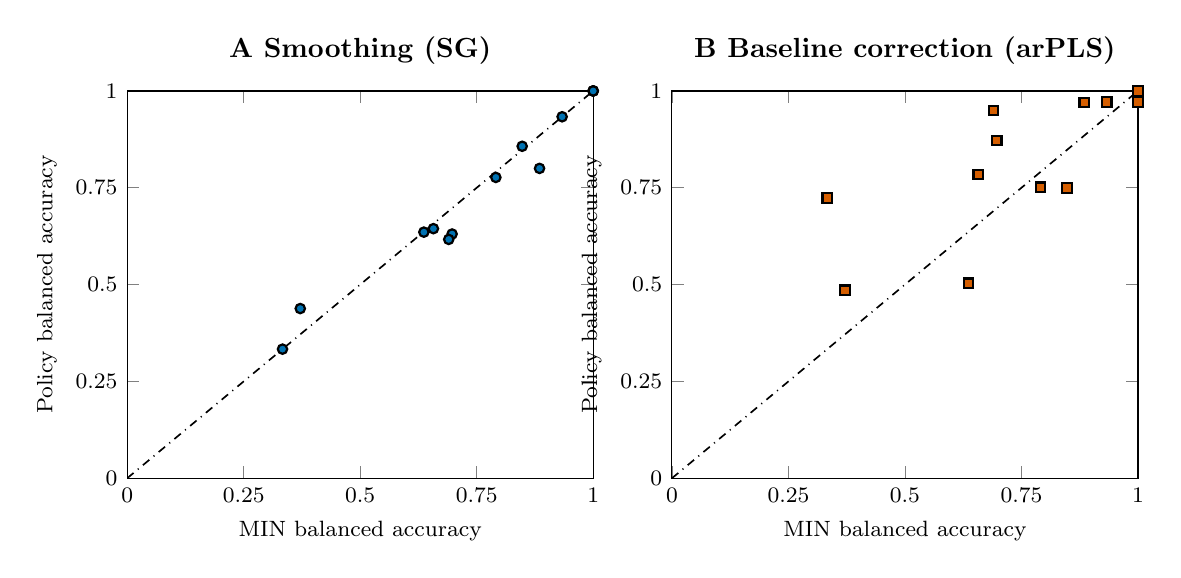
\begin{tikzpicture}
\begin{groupplot}[
  group style={group size=2 by 1, horizontal sep=10mm, vertical sep=6mm},
  width=75mm, height=65mm,
  xmin=0, xmax=1, ymin=0, ymax=1,
  xtick={0,0.25,0.5,0.75,1}, ytick={0,0.25,0.5,0.75,1},
  tick label style={font=\fontsize{8}{9}\selectfont},
  label style={font=\fontsize{8}{9}\selectfont},
  title style={font=\bfseries\fontsize{10}{12}\selectfont},
  xlabel={MIN balanced accuracy}, ylabel={Policy balanced accuracy},
]
\nextgroupplot[title={A  Smoothing (SG)}]
\addplot[black, dash dot, line width=0.6pt, samples=2, domain=0:1, forget plot] {x};
\addplot[only marks, mark=*, mark size=1.7pt, color=f02sg, mark options={draw=black,line width=0.8pt}] coordinates {(0.7911375661375661,0.7767195767195767) (0.6366402116402117,0.6354497354497355) (0.6972222222222222,0.6305555555555555) (1.0,1.0) (1.0,1.0) (0.3333333333333333,0.3333333333333333) (0.9333333333333332,0.9333333333333332) (1.0,1.0) (0.3714285714285714,0.43809523809523815) (0.6571428571428571,0.6444444444444445) (0.884848484848485,0.8) (0.8476190476190476,0.8571428571428573) (0.69,0.6166666666666667)};
\nextgroupplot[title={B  Baseline correction (arPLS)}]
\addplot[black, dash dot, line width=0.6pt, samples=2, domain=0:1, forget plot] {x};
\addplot[only marks, mark=square*, mark size=1.7pt, color=f02arpls, mark options={draw=black,line width=0.8pt}] coordinates {(0.7911375661375661,0.7513227513227514) (0.6366402116402117,0.5035714285714286) (0.6972222222222222,0.8722222222222221) (1.0,1.0) (1.0,1.0) (0.3333333333333333,0.7238095238095238) (0.9333333333333332,0.9714285714285715) (1.0,0.9714285714285715) (0.3714285714285714,0.48571428571428565) (0.6571428571428571,0.784126984126984) (0.884848484848485,0.9696969696969697) (0.8476190476190476,0.7492063492063491) (0.69,0.95)};
\end{groupplot}
\end{tikzpicture}
\par\vspace{4pt}
{\fontsize{8}{10}\selectfont RQ-S01: preprocessing and chemical identification. Source-only selection/calibration; selected CNN identity fixed across policies. SG = impulse replacement, smoothing, minmax; arPLS = impulse replacement, baseline correction, minmax. MIN = minimal minmax. Primary: equal contexts within domain, then equal domains. Pooled-fold sensitivity reconstructs each four-fold prediction set before scoring. M01 individual-spectrum predictions; M06 combined predictions per physical sample. M06 averages model probabilities within sample/instrument then equally across instruments, never input spectra or hard labels. 598 original spectra / 69 physical samples / 10 instruments; 557 spectra in 13 held station/instrument domains, 260 contexts. Per-domain independent support in the CSV/table. D1..D13 are lexicographic station/instrument domains, not samples. Diagonal y=x; the 520 points across all panels are paired domain measurements, not 520 independent observations. Claim limit: cannot establish causal background removal or new-instrument performance; no error bars, no significance stars.}\par
\end{minipage}
\end{document}